\section{Mechanism design}
Since Picolo is an open network and nodes can't be trusted, a robust incentive and disincentive mechanism is required to realize its correct functioning. In this section we discuss how Picolo handles failures and malicious nodes at the database and network layers. Our mechanism design consists of these main pieces:
\begin{enumerate}
	\item Node stakes and incentives
	\item Data availability checks
	\item Paxos based byzantine consensus \cite{byzantine_paxos}
\end{enumerate}
We aim to devise Casper FFG \cite{casper_ffg} style slashing conditions based on the above.
\newline\newline
\textbf{Assumptions in the attack model}: We assume a standard Byzantine failure model, i.e., the attacker is able to make changes to the messages at the network layer on a node or alter the behavior at the database layer. The attacker is also able to coordinate the behavior of multiple nodes in real-time to achieve a desired attack scenario. We also allow for the adversary to delay communication between honest nodes so long as the adversary has the ability to do so given the topology of the overlay network (i.e. the adversary should be part of the routing path). We also assume that the attacker is computationally bound, i.e., they cannot gather enough computing resources to subvert state-of-the-art cryptographic techniques such as Elliptic curve, crypto-hash functions (such as SHA-256) or encryption schemes such as AES.
\newline\newline
\textbf{Node stake}: All nodes in the network need to have a stake in order to have any meaningful participation i.e before they can start hosting large amounts of data. They can either explicitly make a security deposit when they join thereby increasing their stake or can earn rewards overtime by serving large amounts of data (by acting as cache) and use them for making the deposit. While acting as caching nodes, they are not subject to any PoQ checks (\cref{sec:poq}). 
\newline\newline
\textbf{Byzantine behaviour at the database layer}: The central tenet of our design is to use strong cryptographic primitives to push Byzantine behavior at the database layer down to either a DoS style attack vector or to the network layer where we handle it using a combination of crypto-incentives, DHT management and detection. At the database level, each node is responsible for the standard CRUD operations for a given table (or a shard). Each such operation is protected using a cryptographic signature of the entity (dapp or user) that authorizes the request. Thus a malicious node is only able to destroy the data and not alter it. For example, every write request has a signature that certifies the request. Thus, a Merkle proof audit and signature on every table can deter any malicious manipulation of the data stored. The only attack vectors that remain are various versions of DoS style disruption, where a single node or a collection of nodes disrupt the network by delaying messages or destroying the data stored. 
\newline\newline
\textbf{Network level Byzantine behavior}: Here we discuss how to handle attack vectors where the adversary can drop network messages, delete data or both. The routing layer is based on a cryptographic DHT. Thus, it is not possible for the attacker to “choose” to store a particular shard or content. The only way an attacker can do a targeted DoS is by flooding the network with a majority of nodes such that with high probability one of the compromised nodes gets the responsibility for a targeted table or shard. This mapping includes the backup nodes, thus limiting the effectiveness of a targeted attack.
\newline\newline
\textbf{Caching and replication layer incentivizes faster network links and nodes}:
The caching and replication layer prioritizes faster network links and nodes to serve requests. Thus, nodes that are dead, unresponsive or slow will get fewer requests over time. Thus, a DoS style attack scenario will cause diminishing impact over time. While the network adapts to such a disruption, it is possible for the attacker to gain enough stake and temporarily cause a slowdown. However, their stake (or trust level) would go down and they would be responsible for fewer network functions over time essentially degrading their involvement over time.	
\newline\newline
\textbf{Detection}: It is be possible to detect such DoS style behavior quickly at the network layer since the overlay topologies tend to share many links at the layer-3 on the Internet. For example, if a node appears to delay messages at the network level while maintaining fast routes and content availability might indicate malicious intent. The detection “service” can run on the nodes with the maximum stake or trust. They can detect anomalies between different layers of a potentially malicious node and agree to reduce the trust level of that node. Such a detection service can only be thwarted if the malicious node coordinates its behavior across all observable metrics such that it appears as if it is naturally faulty. For this case, it is indistinguishable from a genuinely faulty node for all practical purposes which is handled at the DHT layer (node addition, deletion, failure modes).

\subsection{Data availability checks} \label{sec:poq}
All peers (replicas) in a database cluster constantly ping each other (once every 10 seconds) to check if they are still reachable from one another. These checks are important to ensure that the replication factor of data is always maintained and for automatic fail-over. Normally, these pings contain short meaningless data. We enhance these pings with random checks for actual data nodes are supposed to be storing. We term this \textit{Proof-of-Query (PoQ)} and nodes can prove that they are storing and serving data correctly by responding satisfactorily to PoQ pings. There are two types of PoQs: \textit{peer-PoQ or pPoQ} and \textit{client-PoQ or cPoQ} (see \figref{fig:poq})
\newline
\newline
\textbf{pPoQ}: This is the PoQ that peers (replicas) within a cluster send amongst each other. In addition to ping data, peers randomly query other peers for tiny slivers of data (typically a single column value of a row aka a single cell) and compare the results from each peer against one another and with local data. If there are disparities among the results, then the entire row is fetched along with the digital signature of the row and the public key of the signer. If the signature verification fails for the data returned by a peer, then the validating peer publishes that failure as a violation and triggers the slashing condition. Then the violating peer's deposit is slashed, with a reward going to the validating peer.
\newline
\newline
\textbf{cPoQ}: This PoQ works similar to above except that it can be triggered by any client of the network, typically the party most interested in the data hosted by the cluster (a dapp). cPoQ acts as a second level security check in case all the peers in the cluster are complicit. It is up to the clients how frequently they want to send cPoQs, the trade off being data transfer from a cluster (network egress) costs money.
\newline
\newline
\textbf{Source of randomness}: It is important to choose a good source of randomness so as to ensure queries cannot be guessed ahead in time. If one imagines the data set hosted by a cluster as a giant array and the array size is known, a simple secure random number generator that generates numbers between 0 and 1 will work. Verifiers can then simply get the record at index $ \floor{random * size} $
\newline
\newline
\textbf{Note on signatures}: In our current plan signatures are stored per row. So when a row update occurs on a specific column or group of columns, the signature needs to be recreated for the whole row. This involves fetching the whole row, applying the update, creating the signature on the new row and putting back the whole row. The data overhead with this process might prove to be too much. We are evaluating an alternate scheme where signatures are stored per cell instead using a short signature scheme like BLS \cite{bls}. Trade offs between these two schemes need to be more thoroughly evaluated.
\begin{figure}[h!] \centering
	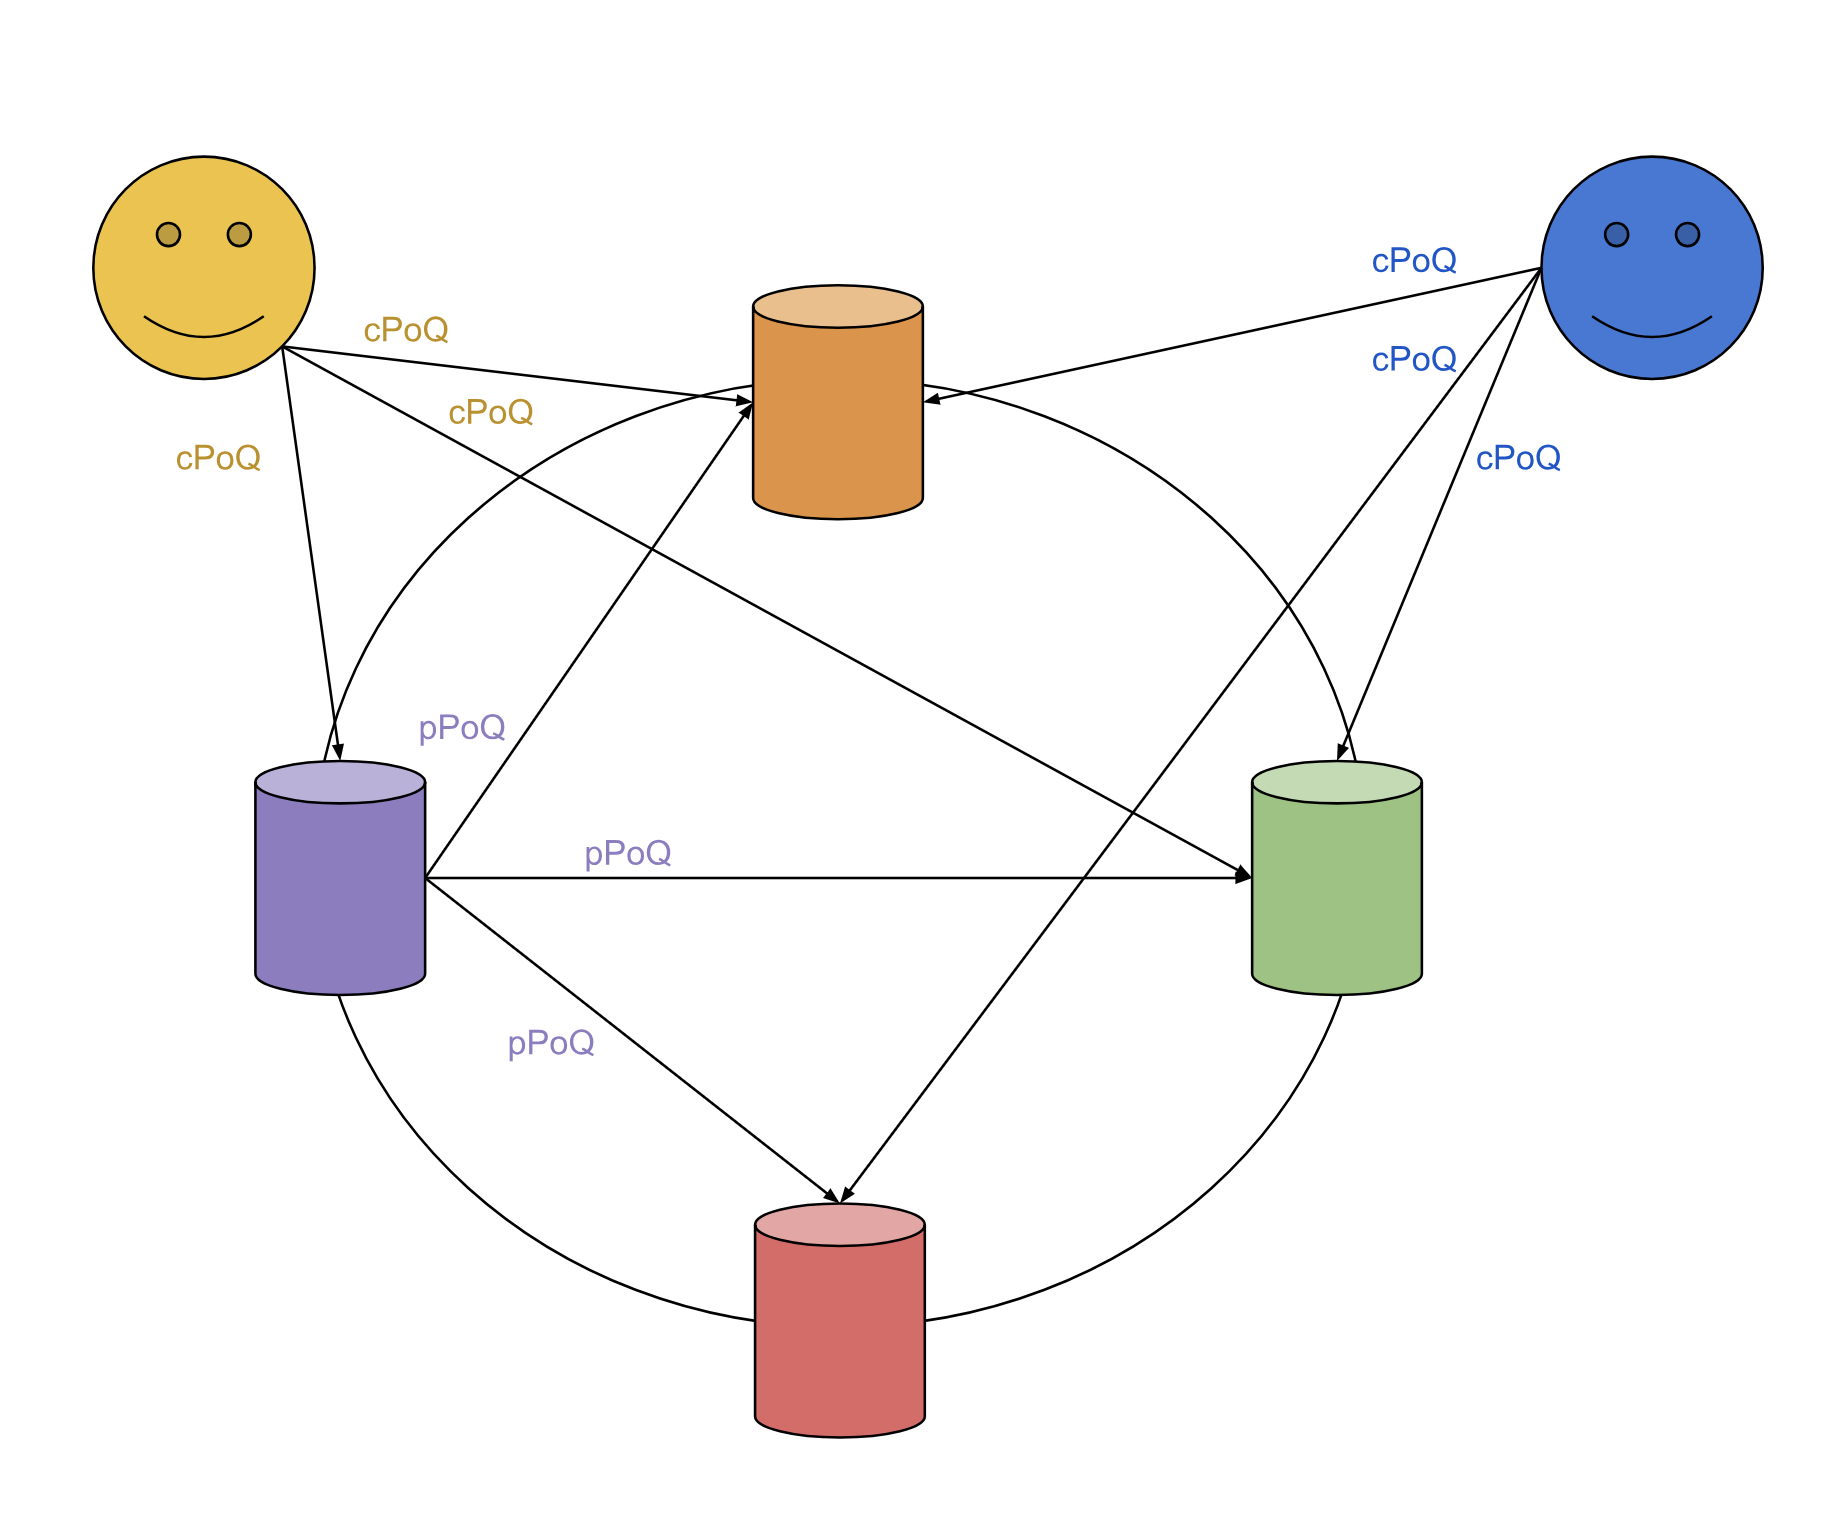
\includegraphics[width=\fscale{1}]{poq.png}
	\caption{Proof-of-Query pings}
	\label{fig:poq}
\end{figure}
 \subsection{Slashing conditions} \label{sec:slashing}
 There are three conditions, meeting any of which will result in the node losing its stake:
 \begin{enumerate}
 	\item Node found to be malicious during a paxos write
 	\item Node is continuously failing PoQ checks
 	\item Node not responding to PoQ checks
 \end{enumerate}
\textbf{Malicious behavior during paxos write}: We use a modified version of generalized byzantine paxos algorithm \cite{byzantine_paxos} for achieving replica consensus (\cref{sec:paxos}). The modified version reports back nodes in the paxos group that behaved arbitrarily during a write to the initiator of the write (client). Client can then issue cPoQs (\cref{sec:poq}) to the reported nodes and check if any data corruption occurred. It may also issue new writes and check if paxos is still reporting back arbitrary behavior of the nodes. It can then publish a proof of arbitrary behavior - simply the wrong query results (that fail signature verification) returned by the malicious nodes to a slashing smart contract that slashes deposits of malicious nodes. Malicious nodes cannot repudiate arbitrary behavior since all messages including responses to cPoQs are digitally signed.
\newline\newline
\textbf{PoQ check failure}: Similar to above, if nodes fail PoQ checks i.e return results whose signatures don't match the respective results, initiator of PoQs can publish proofs to the slashing smart contract to trigger deposit slashing. PoQs can also fail with no data returned due to a genuine hardware failure. In this case more PoQs and calls to collect file system statistics are fired to the node and if these calls indicate hardware failure, the node is simply removed from its paxos group and a replacement will be found. The node can then correct the hardware problem and join a new paxos group or simply choose to withdraw its stake and leave the network.
\newline\newline
\textbf{PoQ check unresponsiveness}: When a node has not explicitly left the network but stops responding to queries, its deposit is slowly drained. Arguably this method is more punitive than is necessary, the alternate being simply marking the node dead and finding a replacement, but stake draining acts as a deterrent to nodes going silent abruptly. It keeps the network more reliable and performant as replacing a node can be an expensive process. The function that calculates draining rate should take into account these factors:
 \begin{enumerate}
	\item Uptime of the node, $t$
	\item Amount of data on the node, $\mathcal{D}$
	\item Current load, $\ell$
	\item Rewards earned so far, $\mathcal{R}$
\end{enumerate}
The function should be inversely proportional to $t$, $\ell$ and $\mathcal{R}$ and directly proportional to $\mathcal{D}$. These relationships make sense because a node with a long uptime might need repair and is genuinely down, a node under heavy load may not be able to respond to PoQs in time as it is busy serving clients, a node that has earned a large amount of rewards so far is trustworthy as it has been serving requests correctly so far and finally since replacing a node hosting a  large amount of data is expensive, it must be penalized for going offline abruptly. Representatively,
\newline
$$ \mathcal{F}_{drain} \propto \frac{\mathcal{D}} {t * \ell * \mathcal{R}}$$
\newline
The exact function to calculate the rate of drain requires more thought and experimental evaluation with some trial \& error and hence not discussed here.

\subsection{Market design}
There are a fixed number of tokens (PINTs - PIcolo Network Tokens), all minted at genesis. They will be distributed according to a well defined plan amongst investors, developers, partners and network participants. The primary economic activity in the network is that the nodes powering the network are paid by consumers for storage, compute and network bandwidth. And the goal of our market design is to optimize towards a single goal:
\begin{center}
	\colorbox{oldlace}{\textit{\large{\textbf{Value of PINTs should increase with usage of the network}}}}
\end{center}
To that end, we propose the following mechanisms:
\subsubsection{Work token model}
In the utility token model, tokens suffer from the velocity problem. The model also requires that tokens be widely distributed aka into the hands of the consumers which could prove difficult to achieve in practice. Mandating the use of network token to pay for services also introduces friction. The user has to convert fiat to ETH/BTC first, then convert them again to the network token on a different exchange. Providers on the other hand need to again convert these tokens into more mature/liquid tokens in order to realize gains as quickly as possible as the cost of them holding on to these tokens could be higher than they like \cite{moe}. 
\newline\newline
To avoid these problems we use the work token model \cite{new_model_utility_token}: network tokens are only required for storage providers to earn the right to join the network. Anyone wishing to become a node on the network need to put up a stake in PINTs in proportion to the resources they'd be providing - more storage provided means more stake required. This stake will be slashed if they are found to be byzantine (\cref{sec:slashing}).They can then accept payment from users in any form they prefer including in PINTs. This token model also captures the value created by the network 100 \% - when the demand for the network goes up, more providers will want to join the network by purchasing PINTs to use as stake. This puts an organic upward price pressure on the token and vice-versa.
\subsubsection{Fair cooperative incentive} \label{sec:fair_incentive}
There are four types of participants in the network (\cref{sec:participants}). The inentives for storage providers and consumers are straight forward - providers get paid by consumers who are benefitting from the service. For the other two types, it is a bit more involved. While the data providers can moentize their data by imposing access controls (\cref{sec:access_control}) and charge for sharing the key information, they might not want to do that. They might be genuinely interested in sharing their data for altruistic purposes or are benefitting in a non-monetary form (e.g: by letting developers create innovative services with the data). But this leads to \textit{free riding} problem and \textit{greedy behavior} amongst nodes. Emmanuelle et. al \cite{fair_incentives} defined the \textit{fair resource sharing} problem and desgined an incentive framework that rewards nodes for acting in a way that maximizes the utility of the network. However, their design depends on a ``middleware layer" that tracks various metrics to properly incentivize and punish nodes. In addition to introducing asymmentry into the network, the tracking mechanism depends on nodes truthfully reporting metrics data. Clearly, this strong assumption will not hold well in a byzantine world as nodes can incorrectly report metrics about their peers in an attempt to damage their participation and access levels defined in \cite{fair_incentives}.
\begin{remark}{\textbf{Reply:}} \label{reply_rule}
	A node should reply to GET messages (\cref{sec:mx_protocol}) if its dataset contains records that satisfy the query in GET message.
\end{remark}
\begin{remark}{\textbf{Forward:}} \label{forward_rule}
	A node should forward GET messages with positive hop numbers to neighbors.
\end{remark}
\begin{definition}{\textbf{Semantic group:}} \label{def:sem_group}
	A semantic group is a dynamic cluster (\cref{sec:dynamic_cluster}) of peers that share semantically similar data.
\end{definition}
\begin{definition}{\textbf{Access level $\mathcal{A}\ell$:}}
	Access level of a node is the probability with which its queries will be fulfilled or other queries will be forwarded to by peers in its semantic group.
\end{definition}
\begin{definition}{\textbf{Cooperative:}}
	A node is said to be cooperative if it follows rule \ref{forward_rule}.
\end{definition}
\begin{definition}{\textbf{Fair:}}
	A node is said to be fair if it follows rules \ref{reply_rule} and \ref{forward_rule}.
\end{definition}
A rational node's objective is to keep its access level high in order to get high quality results to its queries. The access level of each node in a semantic group is tracked by all nodes in the group in a \textit{\textbf{non-interactive}} way i.e a node cannot influence what its peers think the access level of a particular node should be. There is no consensus process amongst nodes to determine a common access level value of a node. Each node determines for itself what the access levels of its peers are based on its past interactions with them. For e.g: if a node $\mathcal{A}$ has responded to a node $\mathcal{B}$'s queries satisfactorily in the past, then $\mathcal{A}$'s access level as far $\mathcal{B}$ is concerned will be high and it will respond to $\mathcal{A}$'s queries favorably in the future. Thus,
\newline
$$ \mathcal{A}_{\mathcal{A}\ell} \propto \sum_{i=0}^{n} \mathcal{N}_i[\mathcal{A}_{a\ell}] + \epsilon$$ 
where $\mathcal{N}_i$ is a node in the semantic group and $\mathcal{N}_i[\mathcal{A}_{a\ell}]$ is $\mathcal{A}$'s access level at that node and $\epsilon$ is a minimum access level all nodes have.
\newline
A new node can elect to increase its access level (the $\epsilon$) by depositing PINTs to a smart contract. Peers check the smart contract when they receive a GET message from this node for the first time and update their local information. Each node maintains three metrics that will help determine the access levels of its peers:
\begin{enumerate}
	\item The number of times a peer $\mathcal{A}$ followed \ref{reply_rule}, $num_{reply}$
	\item The number of times a peer $\mathcal{A}$ followed \ref{forward_rule}, $num_{fwd}$
	\item The ``quality of results" returned by a peer $\mathcal{A}$, $qual (0 < qual < 1)$
\end{enumerate}
$qual$ is loosely defined and its upto to each node how to calculate this value as they are the ultimate consumers of results and its in their best interest to faithfully determine it. Thus, the access level of node $\mathcal{A}$ as per a peer $\mathcal{B}$ can be represented as,
\newline
$$ \mathcal{A}_{a\ell} \propto num_{reply} * num_{fwd} * qual$$
One might notice that there is no explicit definition of a malicious node in this mechanism. This is ok since there is no way in which a node can influence its peers; it may choose to not reply or forward messages from its peers and deliberately set the access levels of its peers to 0 locally but that does not affect the functioning of the semantic group it belongs to. All nodes set the access levels of their peers purely based on their own observation. So its upto each node to choose a behavior aka the manner in which it follows the rules \ref{reply_rule} and \ref{forward_rule} that is best for its purposes.

\subsubsection{Burning games \& applications}
Games that will encourage the burning of PINTs. Since there are a fixed number of them, burning will put an upward pressure on the price. <Todo: Atleast one idea needs to be mentioned here>
Offchain storage network to store contract state. Analytics of on chain data etc.

\subsection{Attacks}
There are four types of participants in the network (\cref{sec:participants}) and a few attacks on/from each of these are discussed below. Storj \cite{Storj} also describes a few attacks that are relevant to a storage network which we touch upon. Below list is by no means exhaustive and we foresee the emergence of a living document in the future dedicated to describing attacks and their mitigations.
\newline\newline
\textbf{Cheating provider}: A storage provider who tries to pretend that they are hosting data without actually doing so. This kind of ``passive" attack is mitigated by cPOQ (\cref{sec:poq}).
\newline\newline
\textbf{Lying consumer}: A storage consumer may report that a provider is failing cPoQs when it actually isn't. To resolve this, consumers are required to report details of the supposedly failed cPoQ, provider information and give read access to the record that cPoQ is supposed to have returned. Then anyone can check whether the cPoQs are actually failing and determine whether to slash the provider's deposit or not. Practically speaking, a committe consisting of other providers is chosen at random to verify this claim and arrives at a consensus \cite{algorand}. 
\newline\newline
\textbf{DDoS on provider}: <solution>
\newline\newline
\textbf{Selective dropper}: A storage provider may selectively drop messages from consumers. If this continues for an extended period, a consumer can simply replace this provider with a new one. Since data is replicated across multiple providers, replacement of one should not create any disruption.
\newline\newline
\textbf{Egregious egress}: A storage provider may untruthfully report serving a shockingly high amount of data to consumers. Since egress earns them money, it is expected that any rational provider tries this attack. <solution>
\newline\newline
\textbf{Free rider}: A peer in a semantic group (\ref{def:sem_group}) may not reply to or forward requests. It just joined the network to gain information about the network like what queries are being sent by clients or gather data from peers while they route it to clients. This attack is mitigated by fair cooperative incentive (\cref{sec:fair_incentive})
\newline\newline
\textbf{Greedy Ganesh}: A peer in a semantic group may choose not to forward any requests to peers or forward them with client information stripped so that they can't reply to clients directly. Then once the peers return results and ask it to route them to a client, it will just combine them with results from its local database and reply to the client as if the whole result set originated from it. Clients then see this peer as a high quality peer and send future requests to it. This leads to the formation of data islands as clients will not being able to discover valuable data hosted by other peers.
\newline\newline
\textbf{Sybil, Google attack, Honest Geppetto}:
\newline\newline
\textbf{Spartacus}:
\newline\newline
\textbf{Eclipse}:
\newline\newline
\textbf{Hostage Bytes}:
\newline\newline
\textbf{Cheating owner}: Micro payments
\newline\newline
\textbf{Faithless farmer}: Non public data should be access controlled via encryption to prevent this attack. (section 5 has more details) 